\subsection{Simulación 1. $\Sigma=0.001$; $T=1K$}

La primera simulación tiene como condiciones iniciales $\Sigma=0.001$; $T=1K$. El resultado de la función de distribución (RDF) se aprecia en la figura (\ref{rdf_0.001_1})

\begin{figure}[t]
	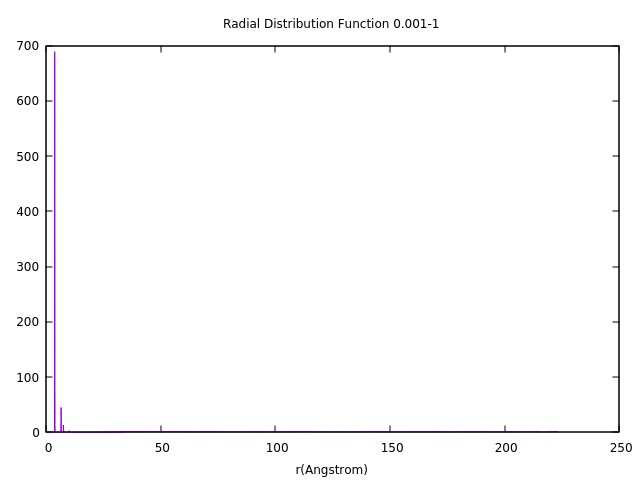
\includegraphics[width=\linewidth]{0.001-1-rdf}
	\caption{Función distribución radial $\Sigma=0.001$; $T=1K$}
	\label{rdf_0.001_1}
\end{figure}

Observamos un pico bastante pronunciado a $r_{1} = 3.81 \textup{\r{A}}$, distancia que corresponde con el valor mínimo (experimental) del potencial de Lennard-Jones, seguido de otros picos inferiores a distancias $r_{3} = 6.59 \textup{\r{A}}$, $r_{2} = 7.63 \textup{\r{A}}$ y $r_{4} = 10.02 \textup{\r{A}}$. Esto indica que los átomos de argón empiezan a agruparse manteniendo dichas distancias entre átomos consecutivos. Efectivamente, la manera más eficiente de agrupar un conjunto de partículas en un sistema bidimensional es a través de un ordenamiento hexagonal, donde las correspondientes distancias $r$ representan las sucesivas distancias entre vecinos más próximos. Así pues $r_{1}=a$ corresponde con la distancia entre un átomo y su vecino más próximo, $r_{2} = 2a$ es la distancia entre el átomo y el segundo vecino más próximo (celda adyacente), $r_{3} = a \sqrt{3}$ para el tercer vecino y finalmente $r_{4}= a\sqrt{7}$ para el cuarto. En la figura (\ref{dist_0.001_1}) se aprecian dichas distancias con un mayor detalle.

\begin{figure}[t]
	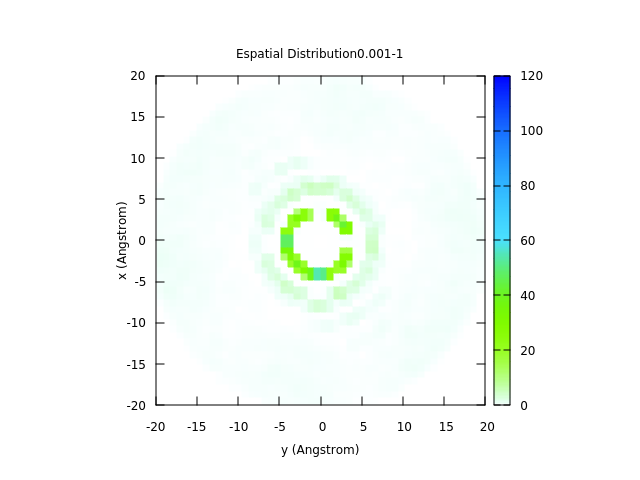
\includegraphics[width=\linewidth]{0.001-1-dist}
	\caption{Distribución a lo largo del plano para $\Sigma=0.001$; $T=1K$}
	\label{dist_0.001_1}
\end{figure}

A medida que aumenta el valor de $r$ el potencial Lennard-Jones tiende a cero y la RDF tiende a 1, lo que en nuestras figuras se traduce en que no se forman aglomeraciones muy grandes en nuestro sistema, lo cual se reafirma teniendo en cuenta que nuestro sistema es muy poco denso y poco energético, es decir, conlleva una mínima interacción entre átomos. Dadas estas circunstancias podemos afirmar que el argón se encuentra en estado sólido.

\subsection{Simulación 2. $\Sigma=0.001$; $T=100K$}

A diferencia que en la simulación anterior, cuando $T=100K$ observamos una dinámica sin conglomerados (clústers) de átomos, pues los átomos tienen suficiente energía cinética como para romper el potencial de enlace dado por Lennard-Jones y por lo tanto son capaces de escapar de su mínimo funcional. Así observamos en la figura (\ref{rdf_0.001_100}) un pico ancho entorno al valor 1 y el correspondiente mínimo de la ecuación (\ref{eq_lennard}) en $r_{1} = 3.81 \textup{\r{A}}$, que muestra como los átomos llegan a formar parejas para inmediatamente después alejarse debido a la alta energía cinética, produciéndose incluso un vaivén entre átomos. En esta situación podemos concluir que el argón se comporta como un gas ideal.

\begin{figure}[t]
	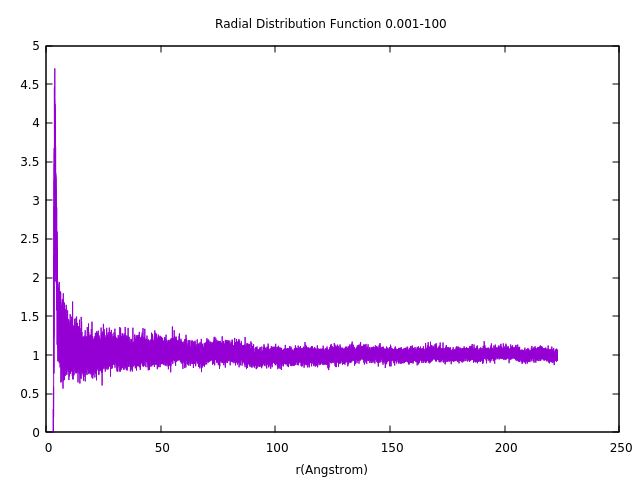
\includegraphics[width=\linewidth]{0.001-100-rdf}
	\caption{Función distribución radial $\Sigma=0.001$; $T=100K$}
	\label{rdf_0.001_100}
\end{figure}

\subsection{Simulación 3. $\Sigma=0.01$; $T=1K$}

En este caso tenemos una situación similar a la dada en la simulación 1. Podemos ver los mismos picos marcados en la RDF, siendo en este caso la figura (\ref{rdf_0.01-1}) la correspondiente para $\Sigma=0.01$; $T=1K$. Como hemos mencionado anteriormente, los valores de $r_i$ son las distancias a los consecutivos vecinos en un conglomerado hexagonal bidimensional, aunque en este caso nos encontramos con más picos debido a la mayor densidad de átomos. El sistema logra un conseguir un estado metaestable con clúesteres de átomos más grandes debido a la baja temperatura. Nuevamente nos encontramos con un comportamiento típico de un sólido cristalino.

\begin{figure}[t]
	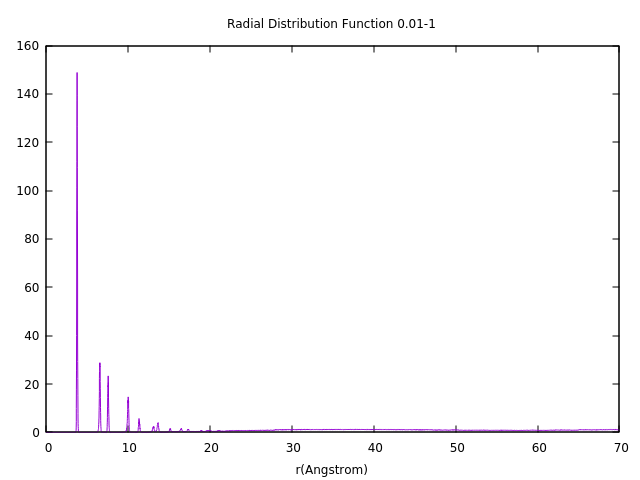
\includegraphics[width=\linewidth]{0.01-1-rdf}
	\caption{Función distribución radial $\Sigma=0.01$; $T=1K$}
	\label{rdf_0.01-1}
\end{figure}

\subsection{Simulación 4. $\Sigma=0.01$; $T=100K$}

La RDF para esta simulación corresponde a la figura (\ref{rdf_0.01-100}). Verificamos un comportamiento similar al de la simulación 2 pero donde la concentración es mayor, es decir, la energía cinética es tal que evita la formación de clústeres. Seguimos observando el mínimo de la ecuación (\ref{eq_lennard}) reflejado en un único pico en la RDF con valor $r_{1} = 3.81 \textup{\r{A}}$ pero relativamente más pequeño. También observamos que la RDF tiende a 1 pero en este caso con un menor ruido, dando lugar a una distribución aún más aleatoria que para la simulación 2.

\begin{figure}[t]
	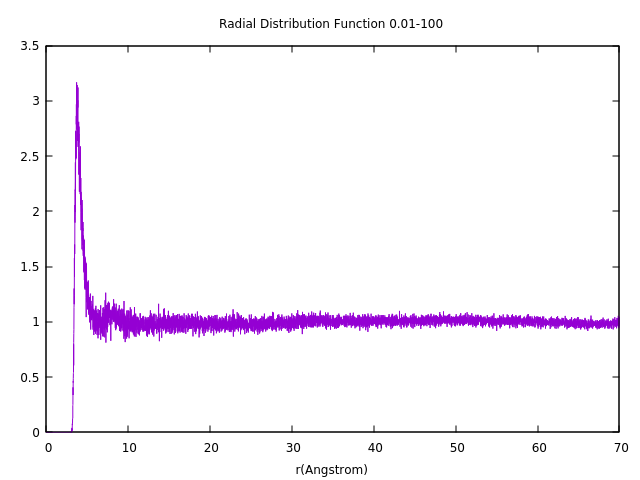
\includegraphics[width=\linewidth]{0.01-100-rdf}
	\caption{Función distribución radial $\Sigma=0.01$; $T=100K$}
	\label{rdf_0.01-100}
\end{figure}

\subsection{Simulación 5. $\Sigma=0.05$; $T=1K$}

La figura (\ref{dist_0.05-1}) para estos valores de densidad y temperatura reflejan un comportamiento típico del estado sólido, con una estructura en clústers de átomos con empaquetamiento no denso. La energía total del sistema recae sobre el potencial de Lennard-Jones según la figura (\ref{figure_lennard}), es decir, la energía cinética es nula y no es posible romper los enlaces atómicos.

\begin{figure}[t]
	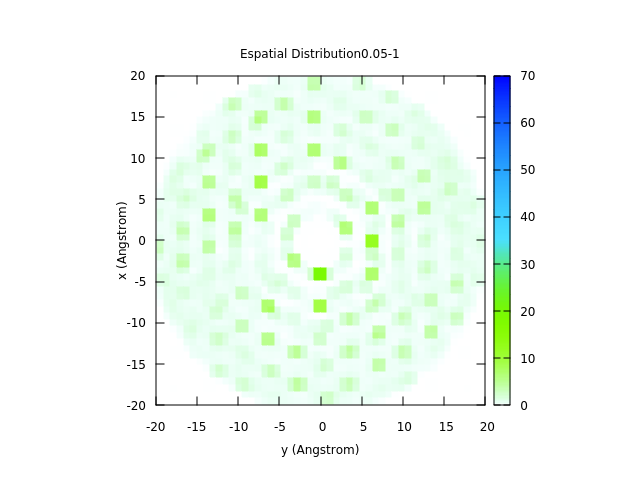
\includegraphics[width=\linewidth]{0.05-1-dist}
	\caption{Función distribución radial $\Sigma=0.05$; $T=1K$}
	\label{dist_0.05-1}
\end{figure}

Podemos ver la misma estructura funcional de la RDF en la figura (\ref{rdf_0.05-1}). Al ser la densidad aún superior que la simulación 1 y 3 observamos más picos en función de $r$. En la figura (\ref{dinamica_0.05-1}) podemos apreciar la estructura compacta del sistema.

\begin{figure}[t]
	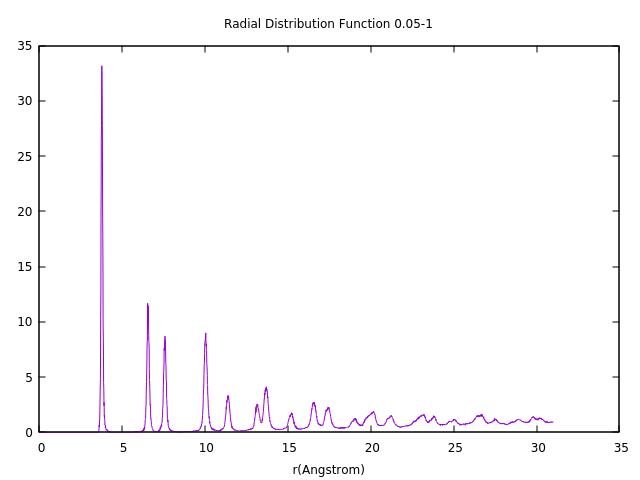
\includegraphics[width=\linewidth]{0.05-1-rdf}
	\caption{Función distribución radial $\Sigma=0.05$; $T=1K$}
	\label{rdf_0.05-1}
\end{figure}

\begin{figure}[t]
	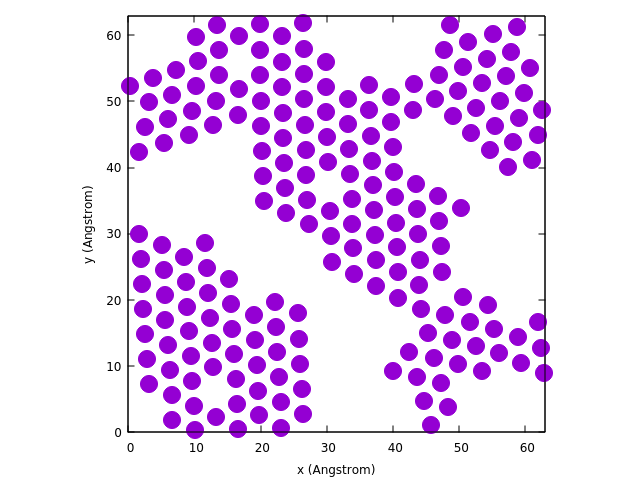
\includegraphics[width=\linewidth]{0.05-1-dinamica}
	\caption{Estructura del sistema al finalizar la simulación $\Sigma=0.05$; $T=1K$}
	\label{dinamica_0.05-1}
\end{figure}

\subsection{Simulación 6. $\Sigma=0.05$; $T=100K$}

En estas condiciones tenemos una RFT en la figura (\ref{rdf_0.05-100}) con los picos ordinarios a una distancia $r$ caracterizada por los consecutivos vecinos, pero siendo éstos picos mucho más anchos. A diferencia que el caso de la simulación 5 ($\Sigma=0.05$; $T=1K$), en el que afirmamos que el argón se encontraba en estado sólido, en este caso tenemos una situación de transición de fase en el que los átomos del sistema empiezan a tener suficiente energía cinética como para romper los enlaces atómicos. Podemos comparar los resultados con respecto a la figura (\ref{dinamica_0.05-100}).

\begin{figure}[t]
	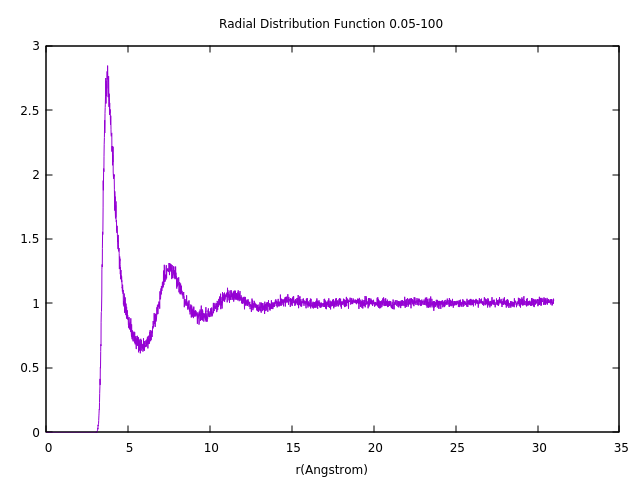
\includegraphics[width=\linewidth]{0.05-100-rdf}
	\caption{Función distribución radial $\Sigma=0.05$; $T=100K$}
	\label{rdf_0.05-100}
\end{figure}

\begin{figure}[t]
	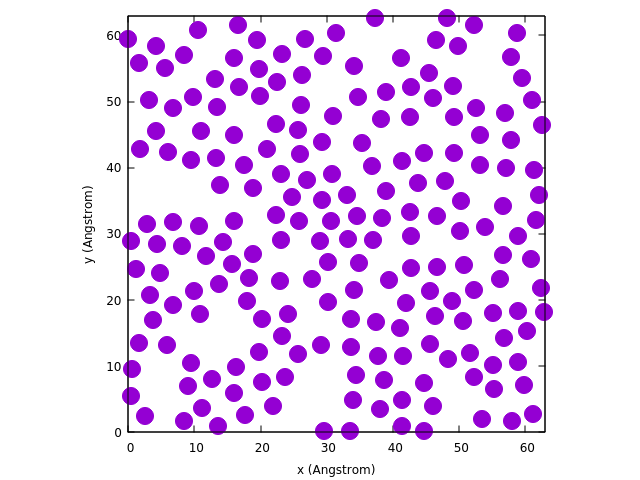
\includegraphics[width=\linewidth]{0.05-100-dinamica}
	\caption{Estructura del sistema al finalizar la simulación $\Sigma=0.05$; $T=100K$}
	\label{dinamica_0.05-100}
\end{figure}

\subsection{Simulación 7. $\Sigma=0.1$; $T= [1,100,1000]K$}

Cuando la densidad es $\Sigma=0.1$ nos encontramos con un caso particular para la RDF no observado anteriormente. En la figura (\ref{rdf_0.1-1}), (\ref{rdf_0.1-100}) y (\ref{rdf_0.1-1000}) podemos ver el resultado de la RDF cuando la temperatura es $T= 1K$, $T= 100K$ y $T= 1000K$, respectivamente. En primer lugar observamos una serie de picos muy agudos a distintas distancias $r$ que no concuerdan con los valores típicos en las simulaciones anteriores. Nuestro valor $r_1$ se ha desplazado a la distancia $3.24\textup{\r{A}}$, al igual que el resto también se ha desplazado a valores inferiores de $r$. Vemos también que han surgido otros picos, siendo la estructura de la RDF en general un poco más ruidosa. Dichos picos se van acampanando a medida que aumentamos la temperatura, son menos ruidosos y se van solapando unos con otros, hasta que a $T=1000K$ la distancia $r$ cobra un comportamiento oscilatorio amortiguado debido al poco espacio que poseen los átomos para recorrer distancias.

Podemos hacer un razonamiento basado en un empaquetamiento de esferas duras para explicar este fenómeno y el por qué, incluso a temperaturas tan altas, observamos un comportamiento de estructura cristalina. En la figura (\ref{dinamica_0.1-1}) podemos visualizar la estructura final. Calcularemos la densidad planar $PN$ del sistema, dado por el cociente entre el número de partículas dentro de una celda y el correspondiente área de la celda. Consideramos una celda hexagonal cuya área es $A_H = 6A_T = 6 \cdot \frac{r^2}{2} \sqrt{3}$, donde $A_T$ es el área de uno de los tríangulos equiláteros que componen la celda hexagonal. Ahora bien, dentro de la celda exagonal caben 3 esferas (contando las porciones de esfera dentro de la celda). Si consideramos $r = \sigma = 3.4 \textup{\r{A}}$ dado que es el valor para el que el potencial de Lennard-Jones es nulo (se trataría del borde de una esfera dura) tenemos que la densidad planar es $PN \simeq 0.09$ partículas$/\textup{\r{A}}^2$, valor que resulta inferior a la densidad del sistema $\Sigma=0.1$ partículas$/\textup{\r{A}}^2$. Esto se traduce en que tenemos una densidad inicial mayor que la posible en un empaquetado de esferas duras con un potenial de Lennard-Jones, lo cual se traduce en términos físicos a un sistema muy compactificado (sometido a mucha presión) donde las partículas apenas tienen posibilidad de moverse y por lo tanto un aumento de temperatura no es suficiente para proveer a los átomos de suficiente energía cinétia como para observar una transición de fase.

\begin{figure}[t]
	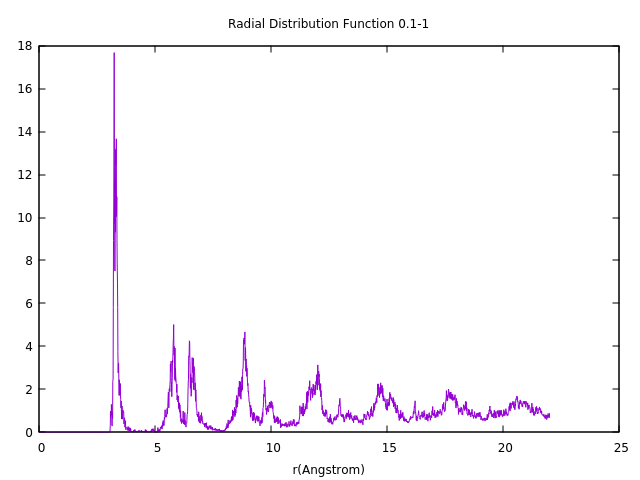
\includegraphics[width=\linewidth]{0.1-1-rdf}
	\caption{Función distribución radial $\Sigma=0.1$; $T=1K$}
	\label{rdf_0.1-1}
\end{figure}

\begin{figure}[t]
	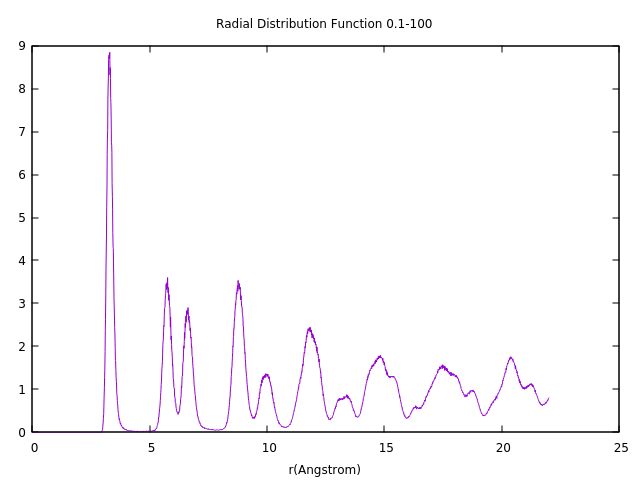
\includegraphics[width=\linewidth]{0.1-100-rdf}
	\caption{Función distribución radial $\Sigma=0.1$; $T=100K$}
	\label{rdf_0.1-100}
\end{figure}

\begin{figure}[t]
	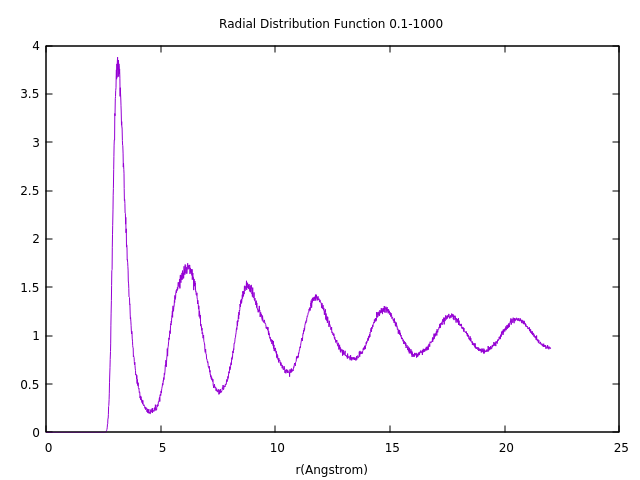
\includegraphics[width=\linewidth]{0.1-1000-rdf}
	\caption{Función distribución radial $\Sigma=0.1$; $T=1000K$}
	\label{rdf_0.1-1000}
\end{figure}

\begin{figure}[t]
	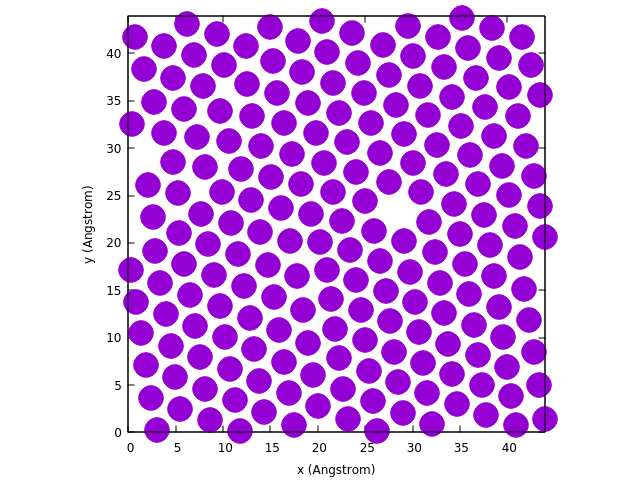
\includegraphics[width=\linewidth]{0.1-1-dinamica}
	\caption{Estructura del sistema al finalizar la simulación $\Sigma=0.1$; $T=1K$}
	\label{dinamica_0.1-1}
\end{figure}

\subsection{Resultados energéticos}

En la figura (\ref{figure_energias}) tenemos una representación gráfica de todas las energías resultantes en las simulaciones. Así podemos hacer un estudio de los resultados energéticos de nuestras simulaciones. Se aprecia como a densidades altas el sistema es capaz de llegar a un equilibrio térmico donde la energía es mínima y estable. Para densidades bajas y temperaturas altas el sistema también llega a un equilibrio térmico y la granuralidad de los datos simplemente es una consecuencia de escala. Recordemos que el estado del argón para estos casos es un estado gaseoso donde cada átomo tiene una energía distinta pero que en su totalidad oscilan entorno a un valor medio dado por la energía total del sistema.

\begin{figure*}[t]
	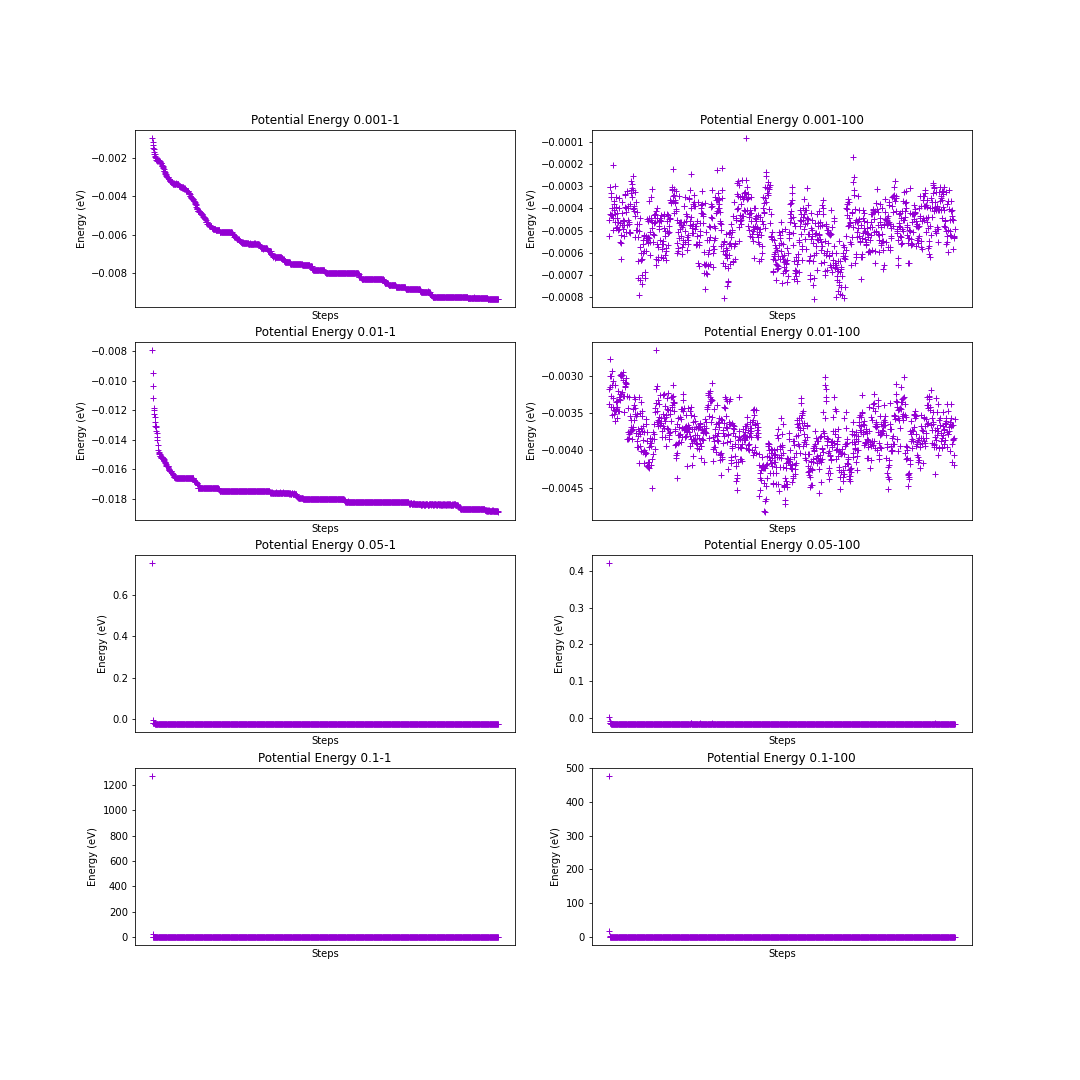
\includegraphics[width=\linewidth,height=20cm]{energias}
	\caption{Energías promedio para los distintos valores de $\Sigma$ y $T$}
	\label{figure_energias}
\end{figure*}

En el caso de densidades y temperaturas bajas vemos como la energía va decreciendo hacia su valor mínimo. En estos casos el sistema no ha tenido tiempo suficiente como para llegar al equilibrio, consecuencia que se refleja en la aparición de clústeres de átomos en la organización del sistema, como si se tratase de un estado metaestable que esta sufriendo una transición.